\documentclass[12pt,preprint]{aastex}

% has to be before amssymb it seems
%\usepackage{color,hyperref}
%\definecolor{linkcolor}{rgb}{0,0,0.5}
%\hypersetup{colorlinks=true,linkcolor=linkcolor,citecolor=linkcolor,
%            filecolor=linkcolor,urlcolor=linkcolor}
%\usepackage{amssymb,amsmath}

\usepackage{color}
\usepackage{url}
\usepackage{graphicx}
\graphicspath{{figures/}}


%\usepackage{listings}
%\definecolor{lbcolor}{rgb}{0.9,0.9,0.9}
%\lstset{language=Python,
%        basicstyle=\footnotesize\ttfamily,
%        showspaces=false,
%        showstringspaces=false,
%        tabsize=2,
%        breaklines=false,
%        breakatwhitespace=true,
%        identifierstyle=\ttfamily,
%        keywordstyle=\bfseries\color[rgb]{0.133,0.545,0.133},
%        commentstyle=\color[rgb]{0.133,0.545,0.133},
%        stringstyle=\color[rgb]{0.627,0.126,0.941},
%    }

\newcommand{\todo}[1]{{\color{red} [TODO: #1]}}
\newcommand{\foreign}[1]{{\it #1}}

\newcommand{\adhoc}{\foreign{ad hoc}}
\newcommand{\etal}{\foreign{et\,al.}}
\newcommand{\etc}{\foreign{etc.}}

\newcommand{\Fig}[1]{Figure~\ref{fig:#1}}
\newcommand{\fig}[1]{\Fig{#1}}
\newcommand{\figlabel}[1]{\label{fig:#1}}
\newcommand{\Eq}[1]{Equation~(\ref{eq:#1})}
\newcommand{\eq}[1]{\Eq{#1}}
\newcommand{\eqlabel}[1]{\label{eq:#1}}
\newcommand{\Sect}[1]{Section~\ref{sect:#1}}
\newcommand{\sect}[1]{\Sect{#1}}
\newcommand{\App}[1]{Appendix~\ref{sect:#1}}
\newcommand{\app}[1]{\App{#1}}
\newcommand{\sectlabel}[1]{\label{sect:#1}}


\begin{document}

\title{Periodograms for Multi-band Astronomical Time Series}

\newcommand{\escience}{1}
\newcommand{\uwastro}{2}
\author{Jacob T. VanderPlas\altaffilmark{\escience}}
\author{{\v Z}eljko Ivezi{\'c}\altaffilmark{\uwastro}}
\altaffiltext{\escience}{eScience Institute, University of Washington}
\altaffiltext{\uwastro}{Department of Astronomy, University of Washington}


\begin{abstract}
This paper introduces the {\it multiband periodogram}, a general extension of the standard 
Lomb-Scargle approach for detecting periodic signals in time-domain data. In addition to 
advantanges of the Lomb-Scargle method such as treatment of non-uniform sampling and
heteroscedastic errors, the multiband periodogram significantly improves period finding for randomly 
sampled multi-band light curves (e.g., Pan-STARRS, DES and LSST). The light curves in 
each band are modeled as arbitrary truncated Fourier series, with the period and phase 
shared across all bands. The key aspect is the use of Tikhonov regularization which drives
most of the variability into the so-called base model common to all bands, while 
fits for individual bands describe residuals relative to the base model and typically require
lower-order Fourier series. This decrease in the required number of fit parameters is the
main reason for improved performance. We use simulated light curves 
and randomly subsampled SDSS Stripe 82 data to demonstrate the superiority of this 
method compared to other methods from the literature. The python implementation of 
this method  is made publicly available as part of the astroML distribution. 
\end{abstract}

\keywords{
    methods: data analysis ---
    methods: numerical ---
    methods: statistical
}

\section{Introduction}

Many types of variable stars show periodic flux variability \citep{EM2008}. Periodic variable stars are important 
both for testing models of stellar evolution and for using such stars as distance indicators (e.g., Cepheids 
and RR Lyrae stars). One of the first and main goals of the analysis is to detect variability and to estimate the 
period and its uncertainty. A number of parametric and non-parametric methods have been proposed to 
estimate the period of an astronomical time series \citep[e.g.,][and references therein]{Graham13}.

The most popular non-parametric method is the phase dispersion minimization (PDM) introduced by \cite{PDM1978}. 
Dispersion per bin is computed for binned phased light curves evaluated for a grid of trial periods. The best
period minimizes the dispersion per bin.  A similar and related non-parametric method that has been recently 
gaining popularity is the Supersmoother routine \citep{Reimann94}. It uses a running mean or running linear 
regression on the data to fit the observations as a function of phase to a range of periods. The best period 
minimizes a figure-of-merit, adopted as weighted sum of absolute residuals around the running mean. 
Neither the Supersmoother algorithm nor the PDM method require a priori knowledge of the light curve shape. 
We note that neither method produces posterior probability distribution for the period but rather a single point 
estimate. 

The most popular parametric method is the Lomb-Scargle periodogram (discussed in detail in \S~\ref{sec:periodograms}.
The Lomb-Scargle periodogram is related to the $\chi^2$ for a least-square fit of a single sinusoid to data
and can treat non-uniformly sampled time series with heteroscedastic measurement uncertainties. 
The underlying model of the Lomb–Scargle periodogram is nonlinear in frequency and basis functions at different
frequencies are not orthogonal. As a result, the periodogram has many local maxima and thus in practice the global 
maximum of the periodogram is found by grid search \citep[for details see, e.g.][]{ICVG2014}.
A more general parameteric method based on the use of continuous-time autoregressive moving average (CARMA) model
was recently introduced by \citep{Kelly14}. CARMA models can also treat non-uniformly sampled time series with 
heteroscedastic measurement uncertainties, and can handle complex variability patterns. 

A weakness of the above methods is that they require homogeneous measurements -- for astronomy data, this means 
that successive measurements must be taken through a single photometric bandpass (filter). This has not been a major
problem for past surveys because measurements are generally taken through a single photometric filter 
\citep [e.g. LINEAR,][]{LINEAR1}, or nearly-simultaneously in all bands at each observation \citep [e.g. SDSS,][]{Sesar2010}.
For the case of simultaneously taken multi-band measurements, \cite{Suveges12} utilized the principal component
method to optimaly extract the best period. Their method is essentially a multi-band generalization of the well-known
two-band Welch-Stetson variability index \citep{Stetson1996}. Unfortunately, when data in each band are taken at
different times, the  principal component approach in not applicable. In such cases, past studies have generally relied 
on \adhoc{} methods such as a majority vote among multiple single-band estimates of the 
periodogram \citep[e.g.,][]{Oluseyi12}. 

For surveys that obtain multi-band data one band at a time, such as Pan-STARRS \citep{Kaiser2010} and DES \citep{Flaugher08},
and for future multicolor surveys such as LSST \citep{Ivezic08LSST}, this \adhoc{} approach is not optimal. In order to take 
advantage of the full information content in available data, it would be desirable to have a single estimate of the periodogram 
which accounts for all observed data in a manner which is not dependent on the underlying spectrum of the object. 
We propose such a method in this paper. 

The proposed method is essentially a generalization of the Lomb-Scargle method to 
multi-band case. The light curves in  each band are modeled as arbitrary truncated Fourier series, 
with the period and phase shared across all bands. The key aspect is the use of Tikhonov regularization 
(discussed in detail in \S \ref{regularization}) which drives most of the variability into the so-called base 
model common to all bands, while fits for individual bands describe residuals relative to the base model 
and typically require lower-order Fourier series. This decrease in the required number of fit parameters is the
main reason for improved performance. 

In \S 2, we provide a brief overview of periodograms, including the matrix-based formulation used in this work. 
XXX Finish this paragraph after the paper is nearly completed... 



\section{Brief Overview of Periodograms \label{sec:periodograms}} 

The detection and quantification of periodicity in time-varying signals is an important area of data analysis within modern time-domain astronomical surveys.
For evenly-spaced data, the {\it Schuster periodogram}, introduced in 1905, gives a quantitative measure of the periodicity of data as a function of the angular frequency $\omega$. For data $\{y_k\}_{k=1}^N$ measured at equal intervals $t_k = t_0 + k\Delta t$, the Schuster periodogram, which measures the spectral power as a function of the angular frequency, is given by
\begin{equation}
  \eqlabel{Schuster}
  C(\omega) = \frac{1}{N}\left| \sum_{k=1}^N y_k e^{i\omega t_k} \right|^2,
\end{equation}
and can be computed very efficiently using the Fast Fourier Transform.

Because astronomical observing cadences are rarely so uniform, many have looked at extending the ideas behind the periodogram to work with unevenly-sampled data. Most famously, \citet{Lomb76} and \citet{Scargle82} extended earlier work to define the {\it normalized periodogram}:
\begin{equation}
  \eqlabel{LombScargle}
  P_N(\omega) = \frac{1}{2\,V}\left[
    \frac{\left[\sum_k(y_k - \bar{y})\cos\omega(t_k - \tau)\right]^2}
    {\sum_k \cos^2\omega(t_k - \tau)}
    +
    \frac{\left[\sum_k(y_k - \bar{y})\sin\omega(t_k - \tau)\right]^2}
    {\sum_k \sin^2\omega(t_k - \tau)}
\right],
\end{equation}
where $\bar{y}$ is the mean and $V$ is the variance of the data $\{y_k\}$, and $\tau$ is the time-offset which makes $P_N(\omega)$ independent of a translation in $t$ \citep[see][for an in-depth discussion]{NumRec}. \citet{Lomb76} showed that this offset has a deeper effect: namely, it makes $P_N$ identical to the estimate of harmonic content given a least-squares fit to a single-component sinusoidal model,

\begin{equation}
  \eqlabel{SingleModel}
  d(t) = A\sin(\omega t + \phi).
\end{equation}

This long-recognized connection between spectral power and least squares fitting methods was solidified by \citet{Jaynes87}, who demonstrated that the normalized periodogram of Lomb and Scargle is a sufficient statistic for inferences about a stationary-frequency signal in the presence of Gaussian noise. Building on this result, \citet{Bretthorst88} explored the extension of these methods to more complicated models with multiple frequency terms, nonstationary frequencies, and other more sophisticated models within a Bayesian framework.


\section{Background: Matrix Formalism for Periodograms}

In this section we present a quick quantitative introduction to the least squares fitting formulation of the normalized periodogram of \eq{LombScargle}. We denote $N$ observed data points as
\begin{equation}
  D = \{t_k, y_k, \sigma_k\}_{k=1}^N
\end{equation}
where $t_k$ is the time of observation, $y_k$ is the observed value (typically a magnitude), and $\sigma_k$ describes the Gaussian errors on each value. Without loss of generality we will assume that the data $y_k$ are centered such that the measurements within each band satisfy
\begin{equation}
  \eqlabel{ycentered}
  \frac{\sum_k w_ky_k}{\sum_k w_k} = 0
\end{equation}
where the weights are $w_k = \sigma_k^{-2}$.

\subsection{Stationary Sinusoid Model}

The normalized periodogram of \eq{LombScargle} can be derived from the normalized $\chi^2$ of the best-fit single-term stationary sinusoidal model given in \eq{SingleModel}. To make the problem linear, we can re-express the model in terms of the parameter vector $\theta = [A\cos\phi, A\sin\phi]$ so that our model is
\begin{equation}
  \eqlabel{simplemodel}
  y(t|\omega,\theta) = \theta_1\sin(\omega t) + \theta_2\cos(\omega t).
\end{equation}
For a given $\omega$, we can find the maximum likelihood estimate of the parameters $\theta$ by minimizing the $\chi^2$ of the model, which is given by
\begin{equation}
  \chi^2(\omega) = \sum_k \frac{[y_k - y(t_k|\omega,\theta)]^2}{\sigma_k^2}.
\end{equation}
For the single-term Fourier model, it can be shown \citep[See, e.g.][]{ICVG2014} that
\begin{equation}
  \eqlabel{chi2PN}
  \chi_{min}^2(\omega) = \chi^2_0[1 - P_N(\omega)]
\end{equation}
where $P_N(\omega)$ is the normalized periodogram given in \eq{LombScargle} and $\chi^2_0$ is the reference $\chi^2$ for a constant model, which due to the assumption in \eq{ycentered} is simply $\chi^2_0 = \sum_k (y_k/\sigma_k)^2$.


\subsubsection{Matrix Formalism}
The expressions related to the stationary sinusoid model can be expressed more compactly by defining the following matrices:
\begin{equation}
X_\omega = \left[
\begin{array}{cc}
\sin(\omega t_1) & \cos(\omega t_1)\\
\sin(\omega t_2) & \cos(\omega t_2)\\
\vdots & \vdots \\
\sin(\omega t_N) & \cos(\omega t_N)\\
\end{array}
\right];~~
y = \left[
\begin{array}{c}
y_1 \\
y_2\\
\vdots \\
y_N\\
\end{array}
\right];~~
\Sigma = \left[
\begin{array}{cccc}
\sigma_1^2 & 0 &  \cdots & 0\\
0 & \sigma_2^2 &  \cdots & 0\\
\vdots & \vdots &  \ddots & \vdots\\
0 & 0 &  \cdots & \sigma_N^2
\end{array}
\right]
\end{equation}
With these definitions, the model in \eq{simplemodel} can be expressed as a simple linear product: $y(t|\omega,\theta) = X_\omega\theta$, and the model and reference $\chi^2$ can be written

\begin{eqnarray}
  \chi^2(\omega) &=& (y - X_\omega\theta)^T\Sigma^{-1}(y - X_\omega\theta)\\
  \chi^2_0 &=& y^T \Sigma^{-1} y
\end{eqnarray}
The expression for the normalized periodogram can be computed by finding the value of $\theta$ which minizes $\chi^2(\omega)$ via standard methods and plugging the result into \eq{chi2PN} to find
\begin{equation}
  \eqlabel{LombScargle2}
  P_N(\omega) = \frac{y^T\Sigma^{-1}X_\omega~[X_\omega^T\Sigma^{-1}X_\omega]^{-1}~X_\omega^T\Sigma^{-1}y}{y^T\Sigma^{-1}y}.
\end{equation}
We note that this expression is equivalent to \eq{LombScargle} in the homoscedastic case with $\Sigma \propto V I$.


\subsubsection{Simple Period Finding}
\sectlabel{simple_period}

\begin{figure}
  \centering
  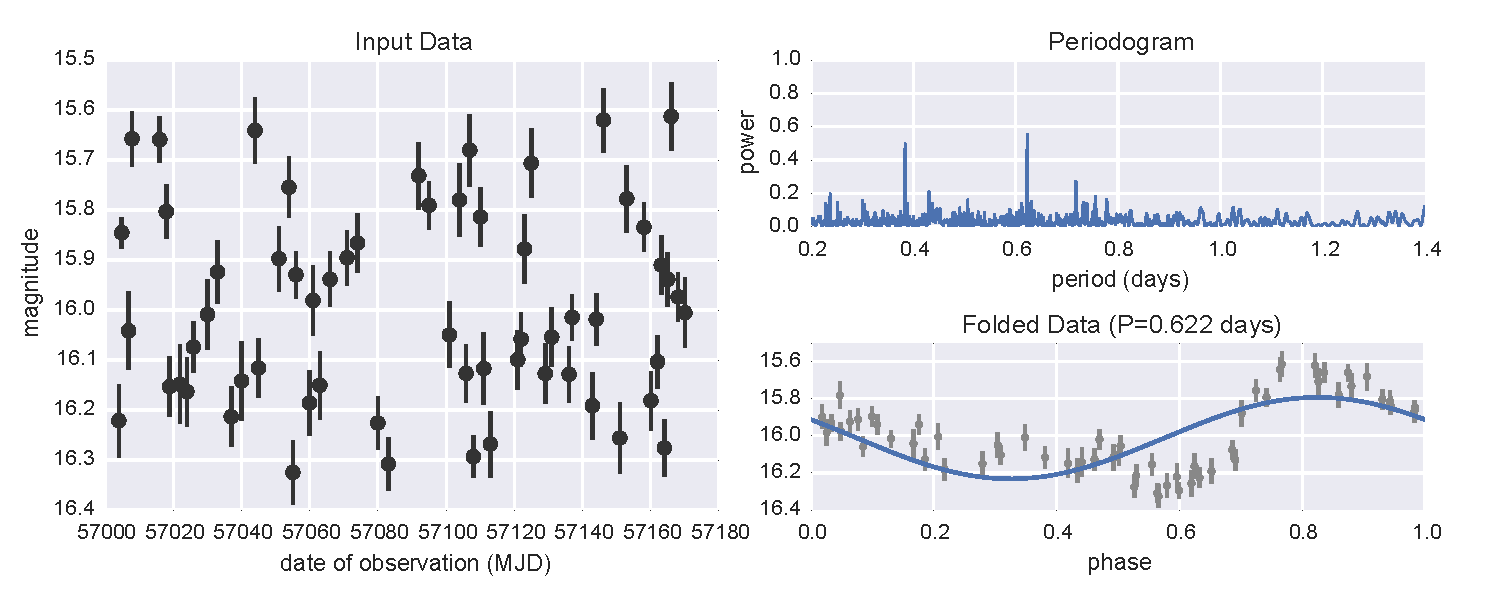
\includegraphics[width=\textwidth]{fig01.pdf}
  \caption{
    An illustration of the basic periodogram and its relationship to the single-term sinusoid model. The left panel shows the input data, while the right panels show the fit derived from the data. The top-right panel shows the periodogram, showing a distinct peak at the true period of 0.622 days, and the bottom-right panel shows the data as a function of phase as defined by this period. Note in the periodogram the presence of the typical aliasing effect, with power located at beat frequencies between the true period and the 1-day observing cadence (see \sect{simple_period} for further discussion).
  }
  \figlabel{basic_example}
\end{figure}

As an example of the standard periodogram in action, we perform a simple single-band harmonic analysis of simulated $r$-band observations of an RR Lyrae light curve, based on empirical templates derived in \citet{Sesar2010} (\fig{basic_example}). The observations are of a star with a period of 0.622 days, and take place on 60 random nights over a 6-month period, as seen in the left panel.

The upper-right panel shows the normalized periodogram for this source as a function of period. While the power does peak at the true period of 0.622 days, an aliasing effect is readily apparent near $P=0.38$. This additional peak is due to beat frequency between the true period $P$ and the observing cadence of $\sim 1$ day. This beat frequency is the first in a large sequence: for nightly observations, we'd expect to find excess power at periods That is, for nightly observations, we'd expect excess power to be found at frequencies $P_n = P / (1 + nP)$ days, for any positive or negative integer $n$. The strong alias in \fig{basic_example} corresponds to the $n=1$ beat period $P_n=0.383$. Though it is possible to carefully correct for such aliasing via the estimated window function \citep[e.g.][]{Roberts87}, we'll ignore this detail in the current work.

The lower-right panel of \fig{basic_example} shows the maximum likelihood interpretation of this periodogram: it is a measure of the normalized $\chi^2$ for a single-term sinusoidal model. Here we visualize the data from the left panel, but folded as a function of phase with the best-fit single-term model over-plot. Here its apparent that the single-term model is biased: RR Lyrae light curves are, in general, much more complicated than a simple sinusoid. Nevertheless, the simplistic sinusoidal model does well is able to recover the correct frequency to a high degree of accuracy (roughly related to the width of the peak) and significance (roughly related to the height of the peak). For a more complete introduction to and discussion of the single-term normalized periodogram, refer to, e.g. \citet{Bretthorst88} or \citet{ICVG2014}.

\subsection{Extending the Periodogram}
We have shown two forms of the classic normalized periodogram: \eq{LombScargle} and \eq{LombScargle2}. Though the two expressions are equivalent, they each have distinct advantages. The expression in \eq{LombScargle} avoids the explicit construction of a matrix, and thus can be computed very efficiently. Furthermore, through some computational tricks taking advantage of the Fast Fourier Transform, expressions of the form of \eq{LombScargle} can be evaluated exactly for $N$ frequencies in $\mathcal{O}[\log{N}]$ time \citep{Press89}.

The matrix-based formulation of \eq{LombScargle2}, though slower than the Fourier-derived formulation, is a more general expression and allows several advantages:
\begin{enumerate}
  \item It is trivially extended to heteroscedastic and/or correlated measurement noise in the data $y_k$ through appropriate modification of the noise covariance matrix $\Sigma$
  \item It is trivially extended to more sophisticated linear models by appropriately modifying the design matrix $X_\omega$.
  \item It is trivially extended to include Tikhonov/L2-regularization (see \S \ref{regularization} for more details)  terms by 
               adding an appropriate diagonal term to the normal matrix $X_\omega^T\Sigma^{-1}X_\omega$.
\end{enumerate}
In the remainder of this section, we'll explore a few of these modifications and how they affect the periodogram and resulting model fits.


\subsubsection{Stationary Sinusoid with Floating Mean}
\sectlabel{floating_mean}

\begin{figure}
  \centering
  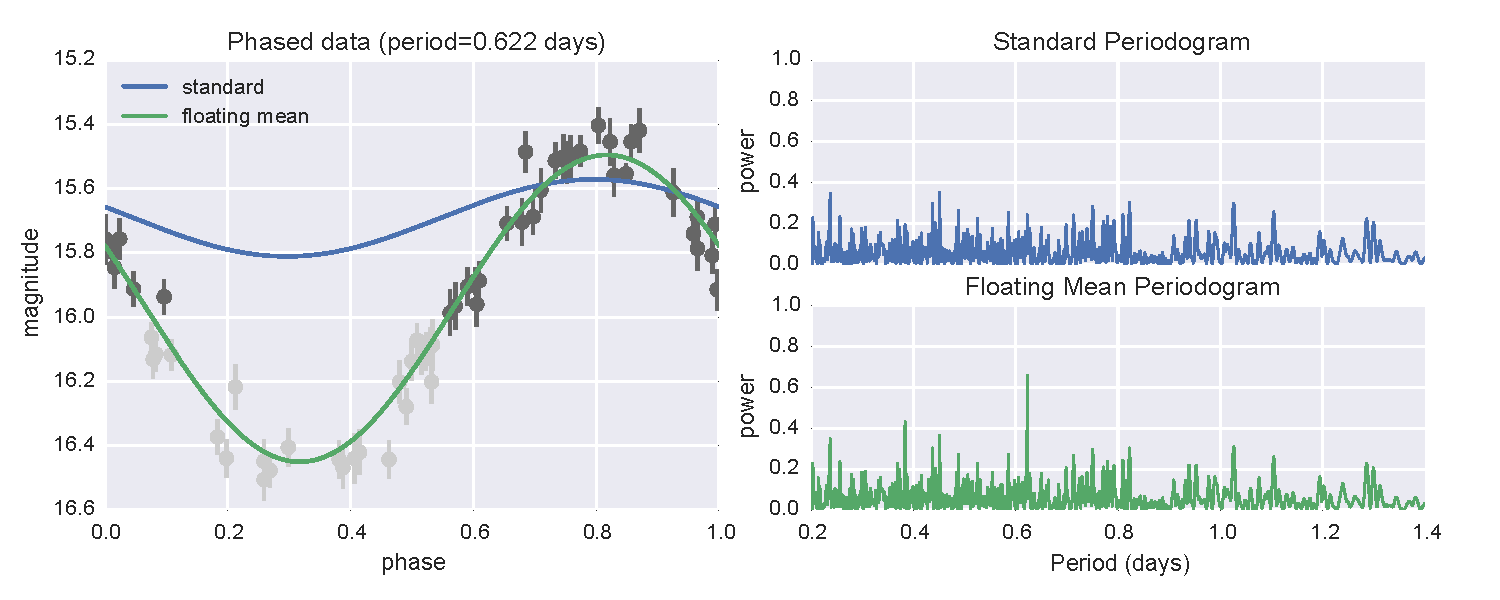
\includegraphics[width=\textwidth]{fig02.pdf}
  \caption{
    An illustration of the effect of the floating mean model for biased data.
    The data consist of 80 observations drawn from a sinusoidal model. To mimick a potentially damaging selection effect, all observations with magnitude fainter than 16 are removed (indicated by the light-gray points). The standard and floating-mean periodograms are computed from the remaining data; these fits are shown over the data in the right panel. Because of this biased observing pattern, the mean of the observed data is not a good predictor of the true mean, and the standard model fails to recover the true period of 0.622 days, while the floating mean model still finds the correct period.
  }
  \figlabel{floating_mean}
\end{figure}

As an example of one of these generalizations, consider the {\it generalized Lomb-Scargle} method of \citet{Zechmeister09}. This adjusts the classic normalized periodogram by allowing the mean of the model to be fit alongside the amplitudes:
\begin{equation}
  y(t~|~\omega, \theta) = \theta_0 + \theta_1\sin\omega t + \theta_2\cos\omega t
\end{equation}
This model can be more accurate than the standard periodogram for certain observing cadences and selection functions. \citet{Zechmeister09} detail the modifications required to the harmonic formalism of \eq{LombScargle} to allow the mean to float in the model. In the matrix formalism, the modification is much more straightforward: all that is required is to add a column of ones to the $X_\omega$ matrix before computing the power via \eq{LombScargle2}.

For well-sampled data, there is usually very little difference between a standard periodogram and a floating-mean periodogram. Where this becomes important is if selection effects or observing cadences cause there to be preferentially more observations at certain phases of the light curve: a toy example demonstrating this situation is shown in \fig{floating_mean}. The data are drawn from a sinusoid with Gaussian errors, and data with a magnitude fainter than 16 are removed to simulate an observational bias (right panel). Because of this selection effect, the mean of the observed data are a poor predictor of the true mean, causing the standard fixed-mean method to poorly fit the data. The floating-mean approach is able to automatically adjust for this bias, resulting in a periodogram which readily detects the input period of 0.622 days (lower-right panel).


\subsubsection{Truncated Fourier Models}
\sectlabel{multiterm}

\begin{figure}
  \centering
  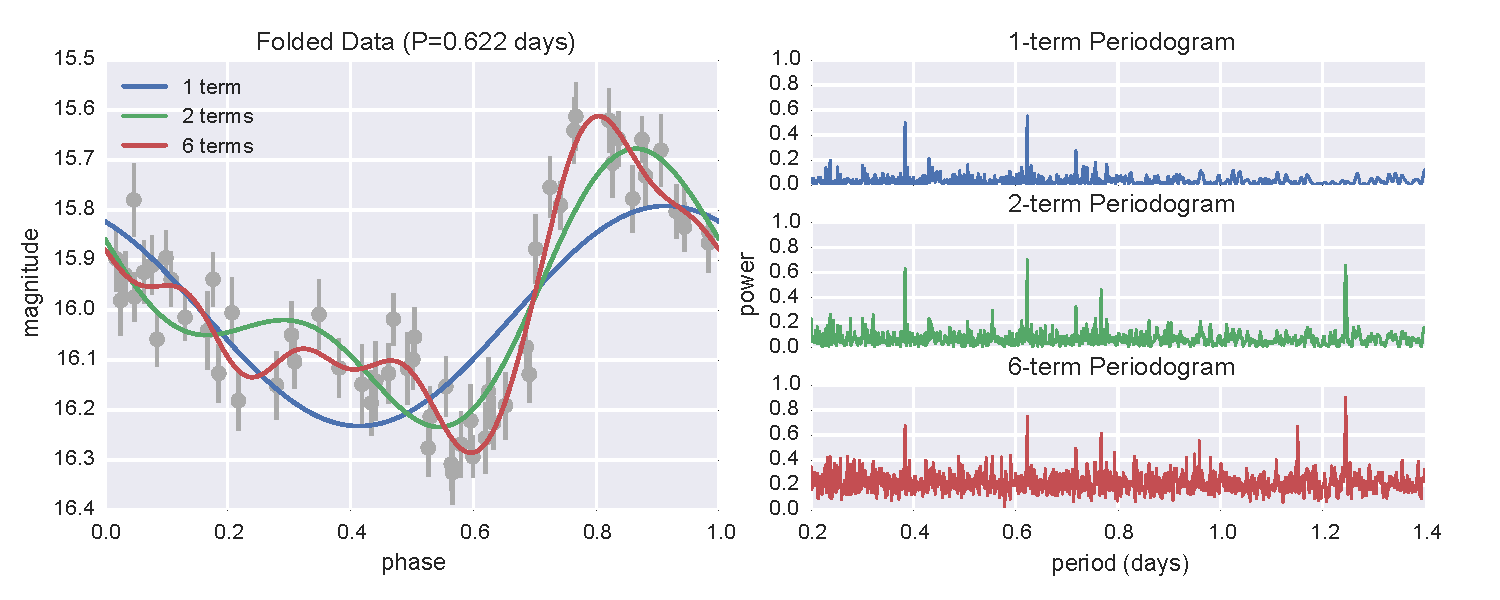
\includegraphics[width=\textwidth]{fig03.pdf}
  \caption{
    An illustration of a periodogram based on the truncated Fourier model.
    The data are the same as those in \fig{basic_example}. Note that the
    higher-order models will show periodogram peaks at multiples of the true
    fundamental frequency $P_0$: this is because for integer $n$ less than
    the number of Fourier terms in the model, $P_0$ is a higher harmonic of
    the model at $P=nP_0$.
  }
  \figlabel{multiterm_example}
\end{figure}

As mentioned above, the standard periodogram is equivalent to fitting a single-term stationary sinusoidal model to the data. A natural extension is to instead use a multiple-term sinusoidal model, with frequencies at integer multiples of the fundamental frequency. With $M$ terms, there are $2M + 1$ free parameters, and the model is given by
\begin{equation}
  y(t|\omega,\theta) = \theta_0 + \sum_{n=1}^M \left[\theta_{2n - 1}\sin(n\omega t) + \theta_{2n}\cos(n\omega t)\right].
\end{equation}
Because this remains a linear model, it can be easily accommodated into the matrix formalism above. For example, an $M = 2$-term floating-mean model can be constructed by building a design matrix $X_\omega$ with $2M + 1 = 5$ columns:
\begin{equation}
X_\omega^{(2)} = \left[
\begin{array}{ccccc}
1 & \sin(\omega t_1) & \cos(\omega t_1) & \sin(2\omega t_1) & \cos(2\omega t_1)\\
1 & \sin(\omega t_2) & \cos(\omega t_2) & \sin(2\omega t_2) & \cos(2\omega t_2)\\
1 & \sin(\omega t_3) & \cos(\omega t_3) & \sin(2\omega t_3) & \cos(2\omega t_3)\\
\vdots & \vdots & \vdots & \vdots & \vdots \\
1 & \sin(\omega t_N) & \cos(\omega t_N) & \sin(2\omega t_N) & \cos(2\omega t_N)\\
\end{array}
\right]
\end{equation}
Computing the power via \eq{LombScargle2} using $X_\omega^{(2)}$ will give the two-term periodogram. As $M$ grows, the size of the design matrix grows, but the periodogram can be computed in the same manner. \fig{multiterm_example} shows a few examples of this multiterm Fourier approach as applied to the simulated RR Lyrae light curve from \fig{basic_example}. There are several important features of this figure that give us insight into the subtleties of this type of multiterm fit.

First, we see in the right panel that all three models show a significant spike at the true period of $P_0 = 0.622$. The higher-order models, however, also show a a spike in power at $P_1 = 2 P_0$: the reason for this is that for and $M>1$-term model, the period $P_0$ is the first harmonic of a model with fundamental frequency $2P_0$, and the higher-order models contain the single-period result.

Second, notice that as the number of terms is increased, the general ``background'' level of the periodogram increases. This is due to the fact that the periodogram is directly related to the $\chi^2$ of the fit at each frequency. Because of the increased model complexity of a higher-order model, it is able to better fit the data at all periods, not just the true period. Thus the observed ``power'' of a higher-order model will be everywhere higher than the power of a lower-order model.

\subsubsection{Regularized Models \label{regularization}}


\begin{figure}
  \centering
  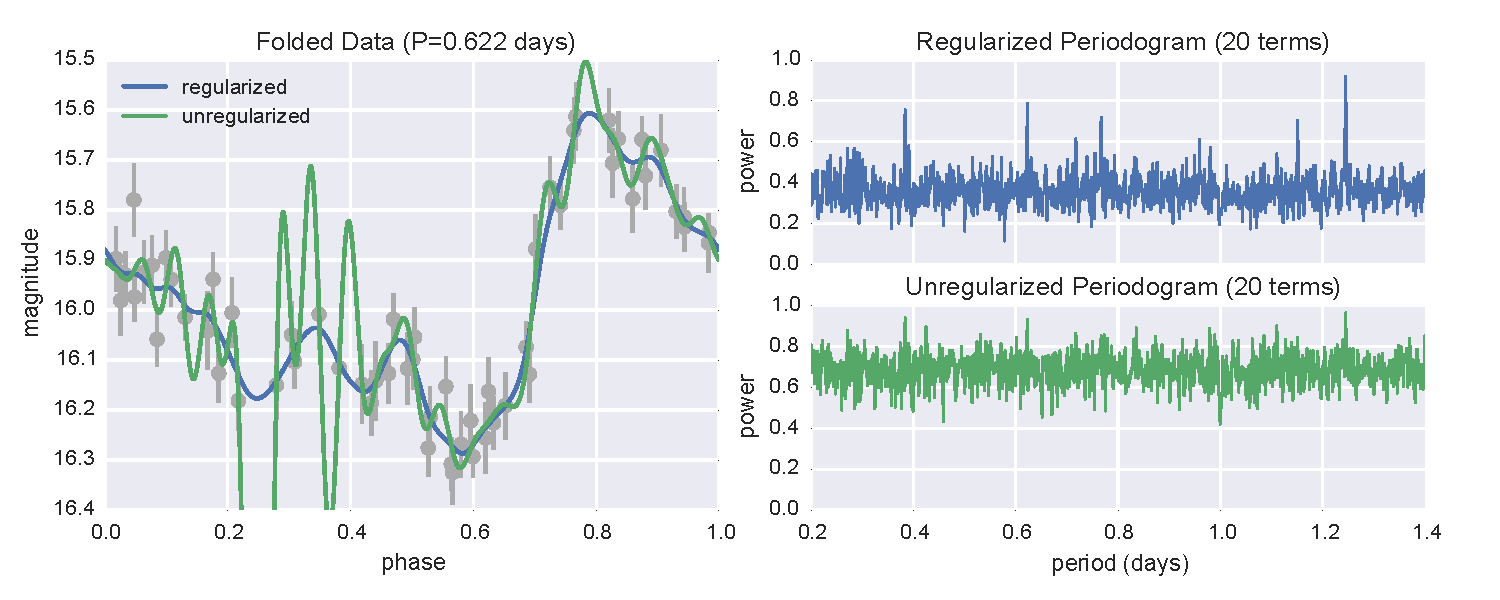
\includegraphics[width=\textwidth]{fig04.pdf}
  \caption{
    The effect of regularization on a high-order model. The data is the same as
    those in \fig{basic_example}. We fit a 20-term truncated Fourier model to
    the data, with and without a regularization term. Without regularization,
    the model oscillates widely to fit the noise in the data. The
    regularization term effectively damps the higher-order Fourier modes and
    removes this oscillating behavior, leading to a model which is much more
    robust to noise in the data.
  }
  \figlabel{regularized_example}
\end{figure}

The previous sections raise the question: how complicated a model should we use? It is easily shown that as we add more terms to the fit, the model will come closer and closer to the observed data. When the number of model parameters equals the number of data points, we can expect to fit the data {\it perfectly} (though in most cases numerical inaccuracies in the fit prevent a truly perfect fit). For very high-order models, the result become very sensitive to the noise in the data, and we say we have {\it over-fit} the data. This can be addressed by explicitly truncating the series, but we can also use a {\it regularization} term to mathematically ensure a less complicated model.

A regularization term is an explicit penalty on the magnitude of the model parameters $\theta$, and can take a number of forms. For computational simplicity here we'll use an {\it L2 regularization} (also known as Tikhonov Regularization), which is a quadratic penalty term in the model parameters added to the $\chi^2$. Mathematically, this is equivalent to the Bayesian approach of using a Gaussian prior on the model parameters.

We encode our regularization in the matrix $\Lambda = {\rm diag}([\lambda_1, \lambda_2 \cdots \lambda_M])$ for a model with $M$ parameters, and our expression for ``regularized'' $\chi^2$ becomes
\begin{equation}
  \eqlabel{chi2reg}
  \chi_\Lambda^2(\omega) = (y - X_\omega\theta)^T\Sigma^{-1}(y - X_\omega\theta) + \theta^T\Lambda\theta
\end{equation}
Minimizing this $\chi^2$, solving for $\theta$, and plugging into the expression for $P_N$ gives us the regularized counterpart of \eq{LombScargle2}:
\begin{equation}
  \eqlabel{LombScargleReg}
  P_N(\omega) = \frac{y^T\Sigma^{-1}X_\omega~[X_\omega^T\Sigma^{-1}X_\omega + \Lambda]^{-1}~X_\omega^T\Sigma^{-1}y}{y^T\Sigma^{-1}y}.
\end{equation}
Notice that the effect of this regularization term is to add a diagonal penalty term to the normal matrix $X_\omega^T\Sigma^{-1}X_\omega$, which has the additional feature that it can correct ill-posed models where the normal matrix is not invertible. This feature of the regularization will become important below.

In \fig{regularized_example}, we compare a regularized and unregularized 20-term truncated Fourier model on our simulated RR Lyrae light curve. We use $\lambda = 0$ on the offset term, and make $\lambda_j$ progressively larger for each harmonic component. The result of the regularized model is less over-fitting to the input data, and a more distinct peaks in the associated periodogram.


\section{A Multiple-Band Model}
To compute a periodogram for multi-band data, we'll take advantage of many of the nice features of the matrix form of the normalized periodogram, which allows us to specify an arbitrary linear model covering our data. We will construct a multi-term Fourier model with the following features:
\begin{enumerate}
  \item An $M_{base}$-term truncated Fourier fit which models a latent parameter, which we'll call the ``overall variability''.
  \item An $M_{band}$-term truncated Fourier fit which models the residual of each band from this overall variability.
\end{enumerate}
The total number of parameters for $K$ filters is then $M_K = (2M_{base} + 1) + K(2M_{band} + 1)$. As a result, for each band $b$ we have the following model of the observed magnitudes:
\begin{eqnarray}
  y_b(t|\omega,\theta) = &\theta_0 + \sum_{n=1}^{M_{base}} \left[\theta_{2n - 1}\sin(n\omega t) + \theta_{2n}\cos(n\omega t)\right]& +\\ 
  &\theta^{(b)}_0 + \sum_{n=1}^{M_{band}} \left[\theta^{(b)}_{2n - 1}\sin(n\omega t) + \theta^{(b)}_{2n}\cos(n\omega t)\right].&
\end{eqnarray}
The important feature of this model is that {\it all bands} share the same base parameters $\theta$, while their offsets $\theta^{(b)}$ are determined individually.

We can construct the normalized periodogram for this model by building a sparse design matrix with $M_K$ columns. Each row corresponds to a single observation through a single band. Columns corresponding to the base model and the matching observation band will have nonzero entries; all other columns will be filled with zeros. For example, the $N_{base}=1$ and $N_{band}=0$ model corresponds to one with a simple single-term periodic base frequency, and an independent constant offset term in each band. The associated design matrix will look as follows:
\begin{equation}
X_\omega^{(1,0)} = \left[
\begin{array}{cccccccc}
1 & \sin(\omega t_1) & \cos(\omega t_1) & 1 & 0 & 0 & 0 & 0\\
1 & \sin(\omega t_2) & \cos(\omega t_2) & 0 & 1 & 0 & 0 & 0\\
1 & \sin(\omega t_3) & \cos(\omega t_3) & 0 & 0 & 0 & 1 & 0\\
1 & \sin(\omega t_4) & \cos(\omega t_4) & 0 & 0 & 1 & 0 & 0\\
\vdots & \vdots & \vdots & & & \vdots & &\\
1 & \sin(\omega t_N) & \cos(\omega t_N) & 0 & 1 & 0 & 0 & 0\\
\end{array}
\right]
\end{equation}
Here the nonzero entries of the final five columns indicate the $ugriz$ band of the given observation: the first row is a $u$-band measurement, the second is a $g$-band, the third is a $i$-band, etc.

From reasoning about the free parameters, or by examining the above matrix it is easy to see that some of the parameters will be degenerate: i.e. $X_\omega$ is low-rank, and the problem is ill-posed. Intuitively, this is due to the fact that if we add an overall offset to the base model, this can be perfectly accounted for by subtracting that same offset from each of the band columns. Mathematically, the result of this is that the normal matrix $X_\omega^T\Sigma^{-1}X_\omega$ will be non-invertible, and thus the periodogram is ill-defined. In order to proceed, then, we'll either have to use a different model, or use a cleverly-constructed regularization term on one of the offending parameters.

We'll choose the latter here, and regularize all the band columns while leaving the base columns un-regularized: for the above matrix, this regularization will look like
\begin{equation}
  \Lambda^{(1,0)} = {\rm diag}([0, 0, 0, \epsilon, \epsilon, \epsilon, \epsilon, \epsilon])
\end{equation}
where $\epsilon$ is some small fraction of the trace of the normal matrix $[X_\omega^T\Sigma^{-1}X_\omega]$. The logic of this choice of regularization is that any component of the model which is common to all bands will be accounted for in the base terms: only components of the fit that differ in each band will affect the band terms. Setting $\epsilon$ to some small fraction of the trace ensures that the regularization effect will be small. With this regularization in place, the model is well-posed and \eq{LombScargleReg} can be used to straightforwardly compute the power. We'll see an example of this in action in \sect{Simulated}.

The final remaining piece to mention is our assumption in \eq{ycentered} that the data are centered. This is required so that the simple form of the reference $\chi^2_0$ remains valid. For the multiband model, this assumption requires that the data satisfy \eq{ycentered} {\it within each band}: equivalently, we could lift this assumption and compute the reference $\chi^2_0$ of the multiband model with an independent floating mean within each band; the results will be identical.

\subsection{Relationship of Multiband and Single-band approaches}
\sectlabel{relationship}
There is a special case of the multi-band approach when $N_{base}=0$ and $N_{band}=1$. In this case, the base offset can be removed completely and the $X$ matrix can be arranged to be block-diagonal. A block-diagonal design matrix in a linear model indicates that components of the model are being solved independently: here the independent components are a standard single-band generalized periodogram within each of the $K$ bands.

For band $k$, we'll denote the single-band normalized periodogram as
\begin{equation}
  P_N^{(k)}(\omega) = 1 - \frac{\chi^2_{min, k}(\omega)}{\chi^2_{0,k}}
\end{equation}
The full multiband periodogram is given by
\begin{equation}
  P_N^{(0,1)}(\omega) = 1 - \frac{\sum_{k=1}^K\chi^2_{min, k}(\omega)}{\sum_{k=1}^K\chi^2_{0,k}}
\end{equation}
and it can easily be shown that the $P_N$ can be constructed as a weighted sum of $P_N^{(k)}$:
\begin{equation}
  P_N^{(0,1)}(\omega) = \frac{\sum_{k=1}^K\left[\chi^2_{0,k}P_N^{k}\right]}{\sum_{k=1}^K\chi^2_{0,k}}.
\end{equation}
This tells us how we can construct a particular case of the multi-term periodogram from a weighted sum of periodograms in each band. Here the weights reflect both how many measurements there are in each band, as well as how much those measurements deviate from a simple constant reference model.

\section{Examples}
Here we'll show several examples of the multiband periodogram method in action.

\subsection{Simulated Example}
\sectlabel{Simulated}

\begin{figure}
  \centering
  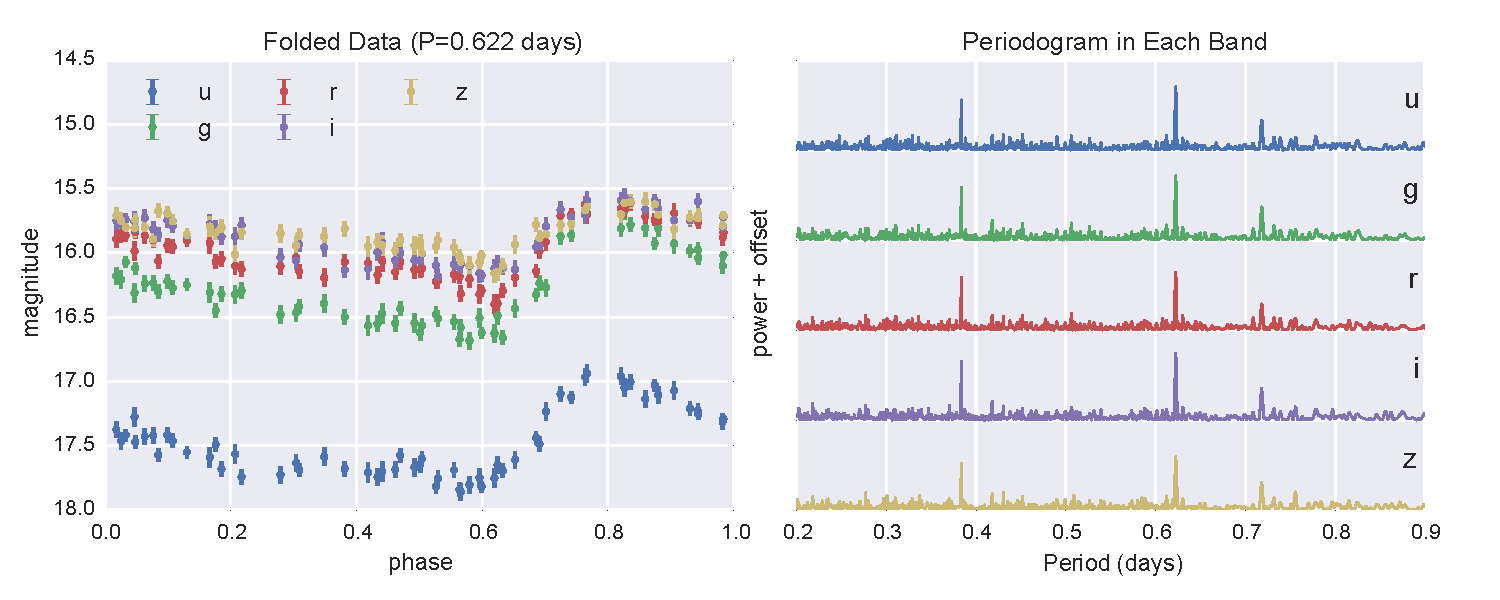
\includegraphics[width=\textwidth]{fig05.pdf}
  \caption{
    An illustration of the typical approach to multiband periodograms,
    in which each band is fit individually. The data consists of 60 coeval
    {\it ugriz} observations spread over 180 nights, and is based on an
    RR Lyrae template from \citet{Sesar2010}. With this much data in each
    band, individual periodograms can be constructed and compared to find the
    true period $P=0.622$ days
  }
  \figlabel{adhoc_example}
\end{figure}


\begin{figure}
  \centering
  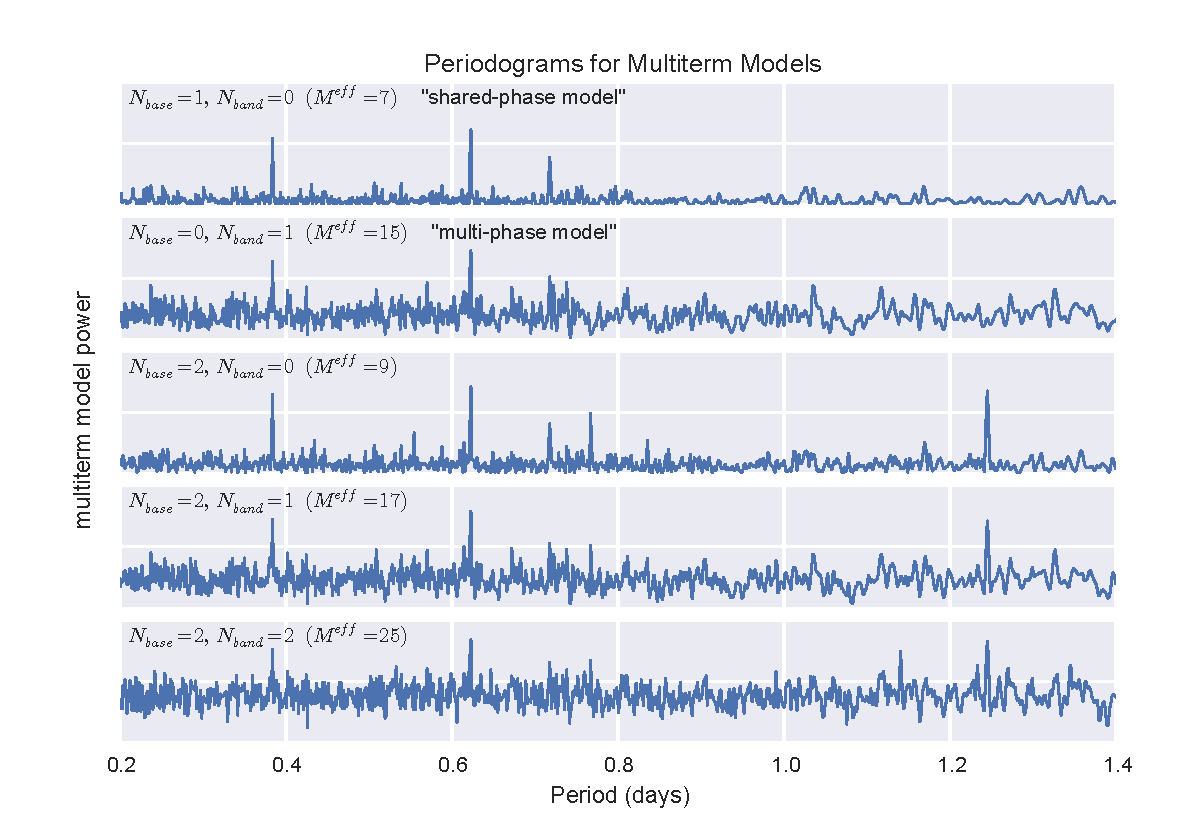
\includegraphics[width=\textwidth]{fig06.pdf}
  \caption{
    Another realization of the data from \fig{adhoc_example}, with only a single
    band observed each night (i.e. 12 observations per band, spread over 180
    days). In this case, single-band data is not sufficient to recover the
    periodogram peaks, and the classic band-by-band approach fails.
    By utilizing all the data at once with the multiband approach
    (with $N_{base}=1,~N_{band}=0$),
    we faithfully reconstruct the periodogram and recover
    the dominant power at period $P=0.622$ days.
  } 
  \figlabel{multiband_sim}
\end{figure}

\todo{We need the bottom-right panel to be bigger! It's our money result! How do we arrange the plot to do this? Also: label it new style and old style.}

\fig{adhoc_example} shows a simulated multiband version of the RR Lyrae light curve from \fig{basic_example}. The observations take place on 60 random nights over a 6-month period, and each night all five bands ({\it u,g,r,i,z}) are recorded. The left panel of \fig{adhoc_example} shows the observations folded as a function of phase.
Using the typical approach from the literature prior to this paper, we individually compute the standard normalized periodogram within each band: the results are shown in the right panel. Here the data is well-enough sampled that a distinct period of 0.622 days can be recognized within each individual band, up to the aliasing effect discussed in \sect{simple_period}.

\fig{multiband_sim} shows the same 60 nights of data, except that each night only a {\it single} band observation is recorded. The left panel again shows the observations as a function of phase, and the right panel shows the periodograms derived from the data. Now, with only 12 observations for each indiviudal band, there is not enough data to accurately determine the period within each single band. With the multiband approach (here computed for $(N_{base},N_{band})=(1,0)$ and $(0,1)$), seen in the lower-right panel of \fig{multiband_sim}, the period is cleanly recovered.

Here we can clearly see the difference between the $(0,1)$ model, which we'll call {\it old-style}, and the $(1,0)$ model, which we'll call {\it new-style}. The old-style model, as discussed in \sectlabel{relationship}, is equivalent to a weighted sum of single-band periodograms for each individual band. The model thus has effectively 15 free parameters, and the phase and amplitude of each band varies individually. As with the truncated Fourier series, this added complexity leads to higher power at off-frequencies. The new-style model, on the other hand, is effectively a 7-parameter model where a single oscillation phase and amplitude is used to describe all of the data. The only flexibility allowed in individual bands is the constant offset. This lower-parameter model produces a periodogram which nicely recovers the input frequency, and has a background level qualitatively similar to that of the single-band observations in \fig{adhoc_example}.


\subsection{Stripe 82}

\begin{itemize}
  \item Compute periods using majority method
  \item Compute periods using unified method
  \item Compare the results
\end{itemize}

\section{Discussion and Conclusion}

\subsection{Further Study}
\begin{itemize}
  \item issues with aliasing \& window function corrections
  \item issues with physicality of model
\end{itemize}


\bibliographystyle{apj}
\bibliography{paper}

%\appendix

\end{document}
